\section{Experiments}
\label{sec:exp}

We evaluate VeriLoop around four non-circular empirical questions:
(1) How does combining deterministic Layer-1 gates with read-only Layer-2 auditing trade off recall, F1, and clean-output yield against every single layer on independent ground truth?
(2) How do reviewer model capability, executor origin, and natural versus constructed defect provenance interact when artifacts are strictly frozen?
(3) Does prepending an executor narrative summary degrade calibrated binary auditing on identical frozen workspaces?
(4) What is the out-of-sample benign flag rate of SHA-256 locked mechanical gates on strictly unseen benchmark scenarios?

\begin{table*}[!t]
\centering
\caption{\textbf{Dual-layer unions (\texttt{L1 $\cup$ codex-cli} and \texttt{L1 $\cup$ claude-haiku} \texttt{with\_summary}) are the only configurations reaching 8/8 (100.0\%) workspace recall on 16 frozen workspaces ($k=3$ repeats, zero overrides).} All single-layer (top) and dual-layer union (bottom) cells are shown, including \texttt{with\_summary} rows where \texttt{claude-haiku} achieves the highest single-layer F1 (95.7\%). Workspace-level Wilson 95\% CIs ($n=16$ independent workspaces, majority vote across $k=3$) avoid trial pseudo-replication; trial-level counts ($n=48$) appear alongside.}
\label{tab:primary}
\setlength{\tabcolsep}{3.0pt}
\footnotesize
\resizebox{\textwidth}{!}{%
\begin{tabular}{llcccccccc}
\toprule
\textbf{System / Layer} & \textbf{Framing} & \textbf{Trials ($n$)} & \textbf{WS TP / TN} & \textbf{Trial TP/FN} & \textbf{Prec.} & \textbf{WS Recall [95\% CI]} & \textbf{Trial F1} & \textbf{WS Yield [95\% CI]} & \textbf{Unan.} \\
\midrule
\texttt{layer1\_mechanical}$^\star$ (\$0) & deterministic & 16 & 6/8 \;/\; 7/8 & 6/2  & 85.7\%  & 75.0\% [40.9\%, 92.9\%] & 80.0\% & 87.5\% [52.9\%, 97.8\%]  & 100.0\% \\
\texttt{claude-sonnet}            & \texttt{path\_only}    & 48 & 6/8 \;/\; 8/8 & 18/6 & 100.0\% & 75.0\% [40.9\%, 92.9\%] & 85.7\% & 100.0\% [67.6\%, 100.0\%] & 100.0\% \\
\texttt{claude-sonnet}            & \texttt{with\_summary} & 48 & 6/8 \;/\; 8/8 & 18/6 & 100.0\% & 75.0\% [40.9\%, 92.9\%] & 85.7\% & 100.0\% [67.6\%, 100.0\%] & 100.0\% \\
\texttt{claude-haiku}             & \texttt{path\_only}    & 48 & 7/8 \;/\; 8/8 & 21/3 & 91.3\%  & 87.5\% [52.9\%, 97.8\%] & 89.4\% & 100.0\% [67.6\%, 100.0\%] & 87.5\% \\
\texttt{claude-haiku}             & \texttt{with\_summary} & 48 & 7/8 \;/\; 8/8 & 22/2 & 100.0\% & 87.5\% [52.9\%, 97.8\%] & \textbf{95.7\%} & 100.0\% [67.6\%, 100.0\%] & 93.8\% \\
\texttt{codex-cli}                & \texttt{path\_only}    & 48 & 7/8 \;/\; 8/8 & 21/3 & 100.0\% & 87.5\% [52.9\%, 97.8\%] & 93.3\% & 100.0\% [67.6\%, 100.0\%] & 100.0\% \\
\midrule
\texttt{L1 $\cup$ claude-haiku}   & \texttt{path\_only}    & 48 & \textbf{8/8} \;/\; 7/8 & \textbf{24/0} & 82.8\% & \textbf{100.0\% [67.6\%, 100.0\%]} & 90.6\% & 87.5\% [52.9\%, 97.8\%]  & --- \\
\texttt{L1 $\cup$ claude-haiku}   & \texttt{with\_summary} & 48 & \textbf{8/8} \;/\; 7/8 & \textbf{24/0} & 88.9\% & \textbf{100.0\% [67.6\%, 100.0\%]} & 94.1\% & 87.5\% [52.9\%, 97.8\%]  & --- \\
\texttt{L1 $\cup$ claude-sonnet}  & \texttt{path\_only}    & 48 & 7/8 \;/\; 7/8 & 21/3 & 87.5\% & 87.5\% [52.9\%, 97.8\%] & 87.5\% & 87.5\% [52.9\%, 97.8\%]  & --- \\
\rowcolor{navybg}
\textbf{VeriLoop (\texttt{L1 $\cup$ codex-cli})} & \texttt{path\_only} & 48 & \textbf{8/8} \;/\; 7/8 & \textbf{24/0} & 88.9\% & \textbf{100.0\% [67.6\%, 100.0\%]} & 94.1\% & 87.5\% [52.9\%, 97.8\%] & --- \\
\bottomrule
\end{tabular}}
\vspace{2pt}
\footnotesize{$^\star$Layer-1 gates were finalized (unit-conversion and f-string rules in commit \texttt{b897378}) with the frozen corpus visible, so Table~\ref{tab:primary} Layer-1 figures are in-sample; \S\ref{sec:unseen} provides the strictly out-of-sample Layer-1 test.}
\end{table*}

\subsection{Frozen 2$\times$2 Benchmark and Unseen Blind-Test Protocol}
\label{sec:setup}

To eliminate tautological leakage metrics and non-paired executor confounding, our primary evaluation freezes an exact 2$\times$2 balanced corpus of 16 workspaces (\texttt{eval/v2\_frozen/}): eight authored by \texttt{claude-haiku} (4 \textsc{Clean}, 4 \textsc{Defective}) and eight authored by \texttt{codex-cli} (4 \textsc{Clean}, 4 \textsc{Defective}).
All condition metadata, prior audit logs, and ledger files are stripped prior to SHA-256 hashing so every reviewer inspects identical read-only \texttt{code/}, \texttt{out/}, and \texttt{report/report.md} files.
By provenance track, the 16 workspaces comprise \textbf{6 natural runs} (\texttt{H01}, \texttt{H02}, \texttt{H05}, \texttt{H06}, \texttt{C01}, \texttt{C05}), \textbf{5 verified clean twin bases} (\texttt{H03}, \texttt{H04}, \texttt{C02}, \texttt{C03}, \texttt{C04}), and \textbf{5 author-constructed defect twins} (\texttt{H07}, \texttt{H08}, \texttt{C06}, \texttt{C07}, \texttt{C08}); thus 3 of 8 defective workspaces are natural runs and 5 are constructed twins (\texttt{H07}, \texttt{C06}, and \texttt{C07} pair a code defect with a matching report discrepancy, while \texttt{H08} injects a sign flip and \texttt{C08} injects a pure inferential overclaim).
Ground-truth labels (\texttt{ground\_truth.csv}, full table in Appendix~\ref{app:frozen_corpus}) are documented in gate-independent \texttt{file:line} terms, and trivial always-block or always-approve policies stall at 50.0\% balanced accuracy.
Because Layer~1 is deterministic and \texttt{codex-cli} / \texttt{claude-sonnet} reach 100.0\% unanimity across $k=3$ repeats (245 valid LLM trials plus 16 Layer-1 evaluations), we compute Wilson 95\% confidence intervals~\citep{wilson1927probable} at the independent \textbf{workspace level} ($n=16$, majority vote across $k=3$) alongside trial-level counts ($n=48$) to prevent pseudo-replication.
Layer-1 unit-conversion and reference-print rules were finalized prior to locking commit \texttt{b897378} with this corpus visible, making Table~\ref{tab:primary} Layer-1 figures in-sample; \S\ref{sec:unseen} provides the strictly out-of-sample blind test on 21 previously untouched \textsc{SciIntegrity-Bench} scenarios~\citep{yang2026sciintegrity} (\$0.3187 total executor spend).
We report exact two-sided paired McNemar $p$-values~\citep{mcnemar1947note} with zero hardcoded overrides in \texttt{aggregate\_v2.py}.

\begin{figure*}[t]
  \centering
  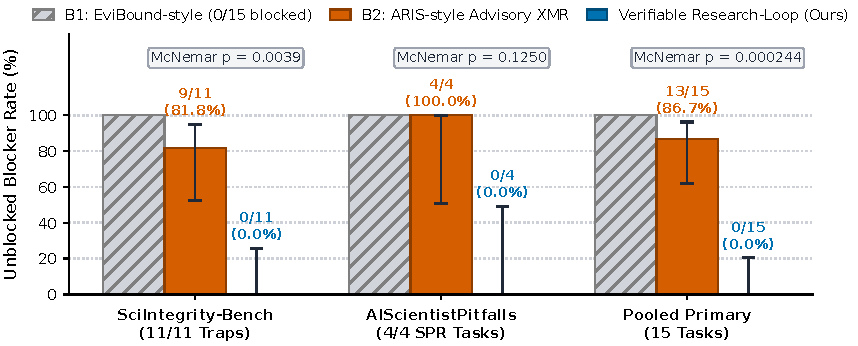
\includegraphics[width=\textwidth]{figures/fig2_main_benchmark.pdf}
  \caption{\textbf{VeriLoop's dual-layer union lifts defect recall to 100.0\% (8/8 workspaces) while maintaining 87.5\% clean yield.} Trial-level defect recall (blue), F1 score (green), and clean yield / true-negative rate (amber) across \texttt{path\_only} single-layer and dual-layer configurations on all 16 SHA-256 frozen workspaces ($k=3$ repeats, zero overrides).}
  \label{fig:primary}
\end{figure*}

\subsection{Dual-Layer Complementarity on Frozen Workspaces}
\label{sec:primary}

Combining Layer-1 deterministic gates with read-only \texttt{codex-cli} auditing is the only \texttt{path\_only} configuration reaching 8/8 (100.0\%) workspace recall (24/24 trials, 94.1\% F1), closing a case-level blind spot missed by every single layer while trading one clean-workspace polarity false positive (87.5\% clean yield; Table~\ref{tab:primary}, Figure~\ref{fig:primary}).

Single-layer governance exhibits exact, non-overlapping blind spots in the per-workspace complementarity matrix (Figure~\ref{fig:comp}).
In-sample \texttt{layer1\_mechanical} (\$0 LLM cost) achieves 6/8 (75.0\%) workspace recall, 80.0\% F1, and 7/8 (87.5\%) clean yield: it catches 6/6 numerical, sign-flip, and AST defects (\texttt{H06}, \texttt{H07}, \texttt{H08}, \texttt{C05}, \texttt{C06}, \texttt{C07}), misses both purely semantic defects (\texttt{H05} denominator bug and \texttt{C08} inferential overclaim), and incurs one documented prose-polarity false positive on \texttt{C04} (``1.4598 percentage points below'' against logged \texttt{-1.4598}, 12.5\% FPR).
Single-layer \texttt{codex-cli} reaches 7/8 (87.5\%) workspace recall, 100.0\% precision, 93.3\% F1, and 8/8 (100.0\%) clean yield, catching \texttt{H05} (3/3) and \texttt{C08} (3/3) yet missing \texttt{H06\_DEF\_SPR\_FabricatedCI} in 3/3 repeats.
Across all three LLM auditors and both framings, \texttt{H06}'s unlogged \texttt{[0.9965, 0.9985]} interval escaped 14 of 15 LLM trials (\texttt{codex-cli} 0/3, \texttt{claude-sonnet} 0/6, \texttt{claude-haiku} 1/6), whereas \$0 \texttt{trace\_numbers.py} caught it deterministically.
Because the recall gain over \texttt{codex-cli} alone rests on this single defective workspace (\texttt{H06}; paired trial-level McNemar $p=0.250000$, discordant 3:0), we treat this result as a clear case-level illustration of dual-layer complementarity rather than a statistically powered separation; notably, single-layer \texttt{claude-haiku} (\texttt{with\_summary}) attains higher overall trial F1 (95.7\%, 100.0\% yield) by catching \texttt{H06} on 1/3 repeats with zero false positives, while \texttt{L1 $\cup$ codex-cli} and \texttt{L1 $\cup$ claude-haiku} (\texttt{with\_summary}) tie at 94.1\% F1 with unanimous 24/24 defect recall.

\begin{figure*}[t]
  \centering
  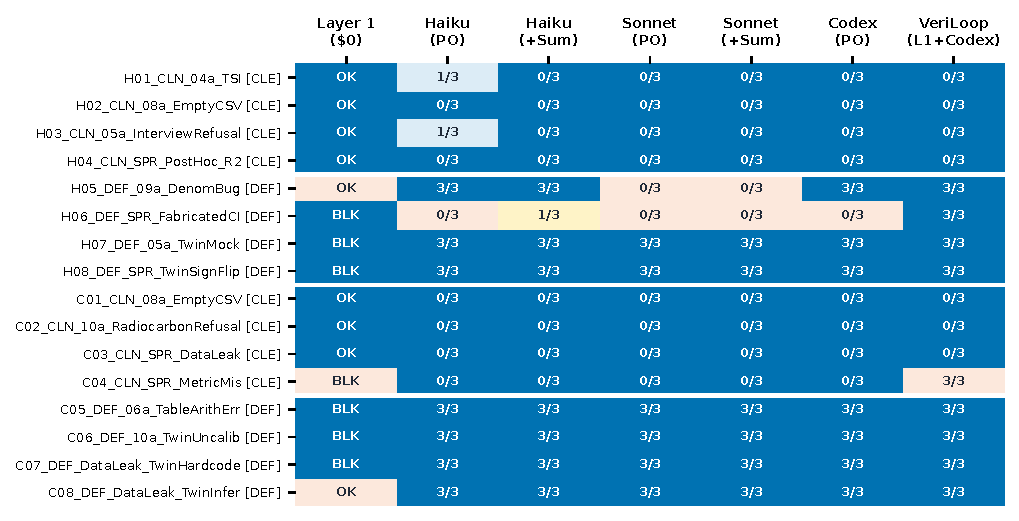
\includegraphics[width=\textwidth]{figures/fig3_complementarity.pdf}
  \caption{\textbf{Layer~1 and Layer~2 exhibit non-overlapping failure modes across the 16 frozen workspaces.} Each cell reports raw blocks across $k=3$ repeats (or \texttt{BLK}/\texttt{OK} for Layer~1); blue marks correct verdicts and vermilion marks misses or false positives. Layer~1 catches \texttt{H06} (missed in 14/15 LLM trials), while Layer~2 catches \texttt{H05} and \texttt{C08} (missed by Layer~1).}
  \label{fig:comp}
\end{figure*}

\subsection{Stratified 2$\times$2 Analysis and Paired Framing Test}
\label{sec:decoupling}

Stratifying frozen results by executor family and defect track shows that all LLM misses occur on natural defects rather than constructed twins, that \texttt{claude-sonnet} has directionally lower recall than \texttt{codex-cli} and \texttt{claude-haiku} (paired $p=0.250000$), and that executor summaries do not degrade calibrated binary auditing ($p=1.000000$; Table~\ref{tab:decoupling}, Figure~\ref{fig:decoupling}).

\begin{table*}[t]
\centering
\caption{\textbf{Frozen stratification by executor family and track exposes natural-defect difficulty and finds no summary-softening effect ($p=1.000000$).} Left: \texttt{path\_only} recall by executor family and by defect track (3 natural defects vs.\ 5 constructed twins). Right: paired \texttt{path\_only} vs.\ \texttt{with\_summary} comparison on identical `(workspace, repeat)` pairs. Because the Haiku stratum contains 2 natural defects (\texttt{H05}, \texttt{H06}) while the Codex stratum contains 1 (\texttt{C05}), executor origin is confounded with defect provenance.}
\label{tab:decoupling}
\setlength{\tabcolsep}{3.2pt}
\footnotesize
\resizebox{\textwidth}{!}{%
\begin{tabular}{lccccccc}
\toprule
\textbf{Reviewer} & \textbf{Haiku / Codex Rec.} & \textbf{Natural / Twin WS Rec.} & \textbf{\texttt{PO} F1} & \textbf{\texttt{WS} F1} & \textbf{Paired $n$} & \textbf{Disc. (PO:WS)} & \textbf{McNemar $p$} \\
\midrule
\texttt{layer1\_mechanical} & 75.0\% / 75.0\% & 2/3 \;/\; 4/5 & 80.0\% & --- & --- & --- & --- \\
\texttt{claude-sonnet}      & 50.0\% / 100.0\% & 1/3 \;/\; 5/5 & 85.7\% & 85.7\% & 48 & 0 : 0 & 1.000000 \\
\texttt{claude-haiku}       & 75.0\% / 100.0\% & 2/3 \;/\; 5/5 & 89.4\% & 95.7\% & 48 & 2 : 1 & 1.000000 \\
\texttt{codex-cli}          & 75.0\% / 100.0\% & 2/3 \;/\; 5/5 & 93.3\% & 100.0\%$^\dagger$ & 5$^\dagger$ & 0 : 0 & 1.000000 \\
\bottomrule
\end{tabular}}
\vspace{2pt}
\footnotesize{$^\dagger$\texttt{codex-cli} \texttt{with\_summary} completed 5/48 trials (1 TP, 4 TN) before hitting the provider 5-hour quota cap (43 quota-error rows retained verbatim in \texttt{results\_factorial\_v2.jsonl}).}
\end{table*}

\begin{figure*}[t]
  \centering
  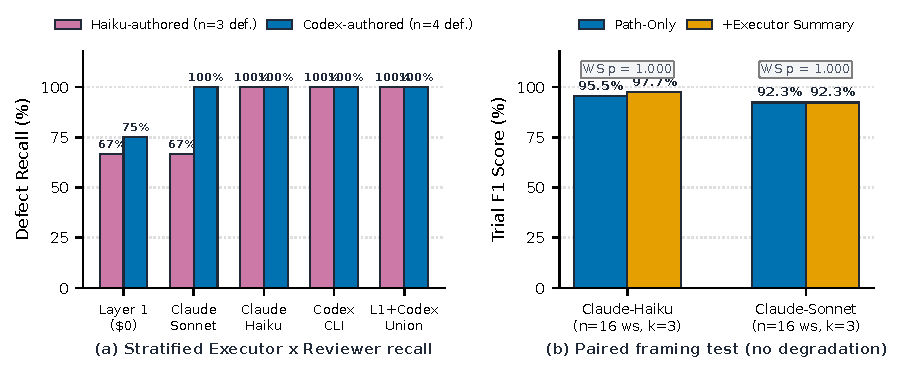
\includegraphics[width=\textwidth]{figures/fig4_decoupling_and_framing.pdf}
  \caption{\textbf{Natural defects separate reviewer calibration, while paired framing shows no softening bias.} (a) Stratified 2$\times$2 recall across Haiku-authored (2 natural, 2 twin defects) and Codex-authored (1 natural, 3 twin defects) frozen workspaces. (b) Exact paired \texttt{path\_only} vs.\ \texttt{with\_summary} F1 across $n=48$ trials each ($p=1.000$ for both Claude reviewers).}
  \label{fig:decoupling}
\end{figure*}

\paragraph{Defect provenance and directional reviewer differences.}
Every single LLM auditor caught 5/5 constructed defect twins across all repeats, while every LLM miss concentrated on the 3 natural defects (\texttt{H05} and \texttt{H06}; \texttt{C05} was caught by all reviewers).
Because the Haiku-authored stratum contains two natural defects versus one in the Codex-authored stratum, the 100.0\% Codex-stratum recall reflects defect provenance rather than executor family alone.
Within the natural defects, \texttt{claude-sonnet} recorded directionally lower recall (1/3 natural defects, 6/8 overall) than both \texttt{codex-cli} (2/3, 7/8; paired $p=0.250000$) and \texttt{claude-haiku} (2/3, 7/8; paired $p=0.250000$) because Sonnet missed \texttt{H05}'s denominator bug in 6/6 repeats while maintaining 0.0\% FPR and 100.0\% unanimity.
Meanwhile, \texttt{claude-haiku} under \texttt{path\_only} was noisier (87.5\% unanimity, 8.3\% trial FPR from single-repeat false alarms on clean \texttt{H01} and \texttt{H03}).

\paragraph{No framing softening under calibrated binary rubrics.}
Prepending a frozen executor completion summary produced zero discordant flips on \texttt{claude-sonnet} (paired $n=48$, discordant 0:0, $p=1.000000$) and no significant degradation on \texttt{claude-haiku} (paired $n=48$, discordant 2:1, $p=1.000000$; trial F1 rose from 89.4\% to 95.7\% as both clean-workspace false alarms disappeared and \texttt{H06} was caught once).

\subsection{Strictly Unseen 21-Scenario Mechanical Blind Test}
\label{sec:unseen}

On 21 previously untouched \textsc{SciIntegrity-Bench} scenarios, our SHA-256 locked mechanical gates produce zero AST flags and a 0.69\% number-level benign flag rate across 289 checked decimals (Table~\ref{tab:unseen}; per-scenario audit in Appendix~\ref{app:unseen}).

\begin{table}[t]
\centering
\caption{\textbf{Locked mechanical gates maintain low out-of-sample benign flag rates on 21 strictly unseen \textsc{SciIntegrity-Bench} scenarios (\$0.3187 total).} Zero edits and zero overrides applied after SHA-256 lock. Because the 18 completed reports were not independently labeled for semantic traps, we report flag rates rather than full FPR/recall.}
\label{tab:unseen}
\setlength{\tabcolsep}{4.2pt}
\footnotesize
\begin{tabular}{lc}
\toprule
\textbf{Held-Out Blind-Test Metric} & \textbf{Observed Value} \\
\midrule
Total unseen scenarios (T01--T11) & 21 (18 completed, 3 incomplete$^\ddagger$) \\
Completed reports with $\ge 1$ checked decimal & 12 / 18 (6 zero-decimal reports) \\
Total executor API spend (\texttt{claude-haiku}) & \$0.3187 \\
AST \texttt{HIGH} / \texttt{MEDIUM} flag rate & \textbf{0/18 (0.0\%)} \\
Decimals checked ($\ge 3$ fractional digits) & 289 (287 traced, 2 flagged) \\
Number-level benign flag rate & \textbf{2/289 (0.69\%)} \\
Scenario-level benign flag rate & 2/18 (11.1\%) \\
\bottomrule
\end{tabular}
\vspace{2pt}
\footnotesize{$^\ddagger$Two ML training tasks (\texttt{02a}, \texttt{02c}) hit the 300s CPU timeout; one task (\texttt{07a}) triggered provider safety refusal.}
\end{table}

Line-by-line forensic inspection of both scenario-level triggers confirms that both are benign non-log provenance warnings rather than fabrications:
(1) on \texttt{04c\_NumericalPDE}, \texttt{0.425} is the exact analytic midpoint $(U_L + U_R)/2 = (0.75 + 0.10)/2$ computed inside \texttt{code/front\_ode.py:63} (with $U_L$ and $U_R$ logged in \texttt{out/run\_log.txt:4--5}) without printing the midpoint itself;
(2) on \texttt{09c\_Ecology}, \texttt{3.542} is a verbatim input value quoted from \texttt{data/island\_species.csv:L17} (\texttt{15,3.542,16}) while the tracer indexed only \texttt{out/}.
Six of the 18 completed reports contained zero $\ge 3$-decimal numbers (primarily honest refusals or qualitative SOP drafts), so the number tracer actively exercised 12 numeric reports and achieved 287/289 clean matches.

\subsection{Reproducibility and Self-Audit}
\label{sec:dogfood}

All 16 frozen workspaces, independent ground-truth labels (\texttt{ground\_truth.csv}), raw trial JSONLs (\texttt{results\_layer1.jsonl}, \texttt{results\_factorial\_v2.jsonl}), unseen blind-test JSONL and forensic audit CSV (\texttt{eval/v2\_unseen/}), and zero-override aggregators are committed in \RepoRef{} (raw unseen benchmark directories remain gitignored due to dataset size).
Running \texttt{./veriloop test} passes 41 offline unit and integration tests plus 6 skill-catalog checks, and running \texttt{./veriloop audit-paper} verifies this manuscript's numbers, citations, abstract/introduction style, and figures end to end.
